\documentclass[oneside]{iitbaps}  %to print on one side of paper
%\setcounter{tocdepth}{4}
%\setcounter{secnumdepth}{4}
% To include optional packages, use the \usepackage command.
% For e.g.:
\usepackage{epsfig}
\usepackage[breaklinks]{hyperref}
\usepackage[all]{hypcap}
\usepackage{amsmath}
\usepackage{amssymb}
\usepackage{svg}
%\usepackage{booktabs}
\usepackage{multirow}
\usepackage{longtable}
\usepackage{hyperref}			
\usepackage{cleveref}
\usepackage{subfig} 
\usepackage{float}
\usepackage{siunitx}
\usepackage{minted}
\usepackage[justification=centering]{caption} 
\usepackage{fancyhdr}


\usepackage[sort&compress]{natbib} %for references

\renewcommand{\vec}[1]{\mathbf{#1}}
\renewcommand{\chaptername}{Assignment}
%=============================================================%
% End of Preamble, start of document


\begin{document}
	

%============================================================================
% prelude.tex
%   - titlepage
%   - dedication (optional)
%   - table of contents, list of tables and list of figures
%   - nomenclature
%   - abstract
%============================================================================


\clearpage%
\pagenumbering{roman}  % This makes the page numbers Roman (i, ii, etc)

%--------------------------------------------------------------------%
% TITLE PAGE
%   - define \title{} \author{} \date{}
\title{CE 605 Applied Statistics}
\author{Ajmal Babu M S}
\date{\today}

%  - Roll number, required for title page, approval sheet, and
%    certificate of course work 
\rollnum{194040007} 

%   - The default report type is preliminary report.
%     For any other type, use  \reporttype{}
%%\reporttype{report-type}
% \aps is a shorthand for \reporttype{progress seminar report}
\reporttype{Assignment Report}
 

%\iitbdegree{Doctor of Philosophy}
%   - The default department is ``Unknown Department''
%     The department can be changed using the command \department{}
\department{Department of Civil Engineering}

%    - Set the guide's name
\setguide{Prof.~Subimal Ghosh}
%    - Set the coguide's name (if you have one)
%%\setcoguide{Prof Amitabha Sanyal}

%   - once the above are defined, use \maketitle to generate the titlepage
\maketitle

%---------------------------------------------------------------------%
%ACCEPTANCE CERTIFICATE
%\makeapproval
\clearpage
%\input{./Chapters/acceptancecertificate}
\clearpage
%--------------------------------------------------------------------%
% ABSTRACT
% \begin{abstract}
% \input{abstract}
% \end{abstract}

%--------------------------------------------------------------------%

%--------------------------------------------------------------------%
%\input{listofsymbols}
% NOMENCLATURE
% \begin{nomenclature}
% \begin{description}
% \item{\makebox[0.75in][l]{$C_1$}} Constant 1
% 
% \item{\makebox[0.75in][l]{$V$}}    Voltage 
% 
% \item{\makebox[0.75 
%\listoffigures
%\listoftablesin][l]{\$}}     US Dollars
% \end{description}
% \end{nomenclature}


%--------------------------------------------------------------------%
%  Single counter for theorems and theorem-like environments:
\newtheorem{theorem}{Theorem}[chapter]
\newtheorem{assertion}[theorem]{Assertion}
\newtheorem{claim}[theorem]{Claim}
\newtheorem{conjecture}[theorem]{Conjecture}
\newtheorem{corollary}[theorem]{Corollary}
\newtheorem{definition}[theorem]{Definition}
\newtheorem{example}[theorem]{Example}
\newtheorem{figger}[theorem]{Figure}
\newtheorem{lemma}[theorem]{Lemma}
\newtheorem{prop}[theorem]{Proposition}
\newtheorem{remark}[theorem]{Remark}

%--------------------------------------------------------------------%
% Make the page numbers Arabic (1, 2, etc)
\tableofcontents 
%\listoffigures
%\listoftables
\cleardoublepage%
\pagenumbering{arabic}



\chapter{Function of Random Variable}

\section{Problem Statement} 

\textit{Show that the sum of two independent identically distributed exponential random variables is a gamma distribution.} \\


Let X and Y be two independent identically distributed exponential random variables with $\lambda=0.15$ \\
Let Z = X + Y \\
Find the pdf of Z, and obtain its parameters by independently generating 1000 values for X and Y

\section{Analytical Solution} 

\begin{align*} 
X &\sim Exp[\lambda]		 &		0 \le X \le \infty \\ 
Y &\sim Exp[\lambda]		 &		0 \le Y \le \infty \\ 
Z &= X + Y		 		&		%0 \le Z \le \infty
\end{align*}
where, \\
X~and~Y~are~independent


\begin{align*} 
X &= Z - Y		 &		0 \le X \le Z \\
\end{align*}

The distribution function for Z, 
\begin{align*} 
f_{Z}(z)	=	\int_{-\infty}^{\infty} f_{X}(x) ~ f_{Y}(z-x) ~ dx \\
			=	\int_{0}^{z} \lambda ~ e^{-\lambda~x} ~ \lambda ~ e^{-\lambda~(z-x)} ~ dx \\
			= \lambda ^2	~	z	~	e^{-\lambda z}
\end{align*}
which is a gamma distribution \\
\begin{align*} 
f_Z(z)&=\frac{\nu(\nu z)^{a-1}}{\Gamma(a)} ~ e^{-\nu z} &  z \ge 0 \\
&=0 	& 	z < 0
\end{align*}

with $a = 2 $ and $\nu = \lambda$

\section{Numerical Solution} 
The problem is solved numerically by independently generating 1000 exponential random variables for X and Y with $\lambda = 0.15$  using Python-based \textit{scipy.stats} library.

\textbf{Obtained parameters for Z are a = 2.0114 and $\nu$ = 0.1482 \\}
The histogram, and PDF are plotted for X, Y and Z as below. \\

\begin{figure}
	\centering
	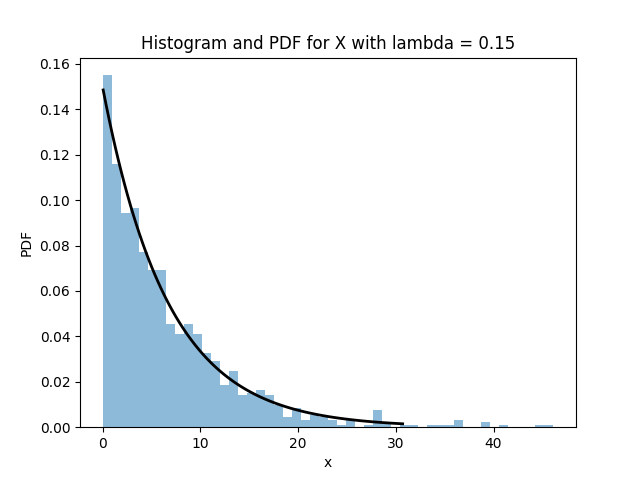
\includegraphics[width=0.9\linewidth]{Figures/Chapter1/Figure_1}
	\caption{Histogram and PDF for X with $\lambda$ = 0.15}
	\label{fig:figure1}
\end{figure}

\begin{figure}
	\centering
	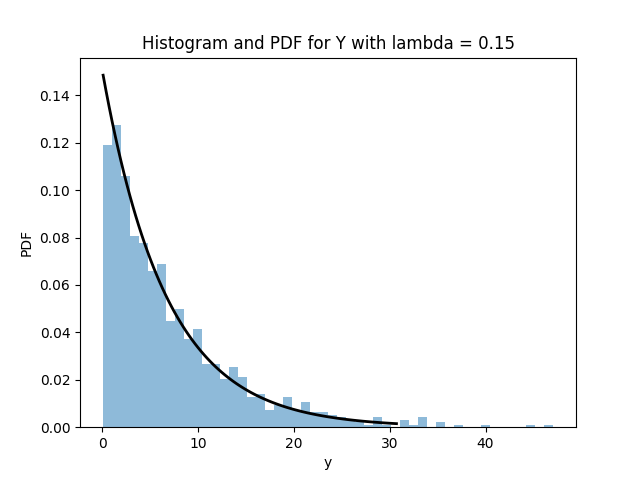
\includegraphics[width=0.9\linewidth]{Figures/Chapter1/Figure_2}
	\caption{Histogram and PDF for Y with $\lambda$ = 0.15}
	\label{fig:figure2}
\end{figure}


\begin{figure}[H]
	\centering
	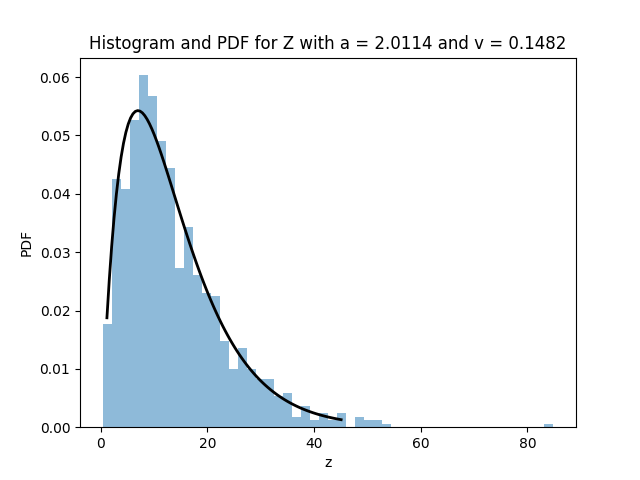
\includegraphics[width=0.9\linewidth]{Figures/Chapter1/Figure_3}
	\caption{Histogram and PDF for Z with a = 2.0114 and $\nu$ = 0.1482}
	\label{fig:figure3}
\end{figure}

The \textit{Python} code used for this computation is given in \ref{Chap:appendix:1}{ Appendix} \\
The source codes are made available in \href{https://github.com/ajmalbabums/ce605assignments.git}{github.com/ajmalbabums/ce605assignments}
%\include{./Chapters/chapter2}
%\include{./Chapters/chapter3} 
%\include{./Chapters/chapter4} 
%\include{./Chapters/chapter5}
%\include{./Chapters/chapter6} 
%\include{./Chapters/chapter7}  
\bibliographystyle{natbib}
%{\small
%\bibliography{Papers}}
\chapter*{Appendix}\label{Chap:appendix}
\addcontentsline{toc}{chapter}{Appendix}

\subsection*{Assignment 1}\label{Chap:appendix:1}

\addcontentsline{toc}{section}{Assignment 1}

 The following python code is made for verifying the sum of two independent identically distributed exponential random variables results a gamma distribution. The input values are the parameter for exponential distribution($\lambda$) and number of random numbers to be generated for the computation. In the current code, $\lambda$ is taken as 0.15 and 1000 random variables are generated.


\inputminted[
frame=lines,
framesep=2mm,
baselinestretch=1.2,
fontsize=\footnotesize,
linenos
]{python}{../assignment1.py}




\end{document}

